\section{Implementation}

Under the NGS regime, candidate solutions will consist of two components:
\begin{enumerate*}[label=(\arabic*)]
\item a raw architectural configuration $A$, and
\item a vector $v$ of network pruning parameters.
\end{enumerate*}
These components will be encoded and recombined separately using standard neuroevolution and genetic algorithm techniques, respectively.
To evaluate a candidate solution, the connection weights of the raw architectural configuration $A$ will be trained for a fixed number of iterations.
Then, a pruning decision will be made for each network node by comparing a quadratic weighting (defined by $v$) of the following metrics to a fixed cutoff value (also defined by $v$):
\begin{enumerate*}[label=(\alph*)]
\item node activation,
\item correlation of node activation with activation of afferent nodes,
\item correlation of node activation with loss, and
\item magnitude and sign of backpropagation gradient through the node.
\end{enumerate*}
Following pruning, training will resume for a fixed number of iterations. Candidate solution fitness will be assessed as the validation set performance of the final trained network.
\begin{minipage}{0.8\textwidth}
 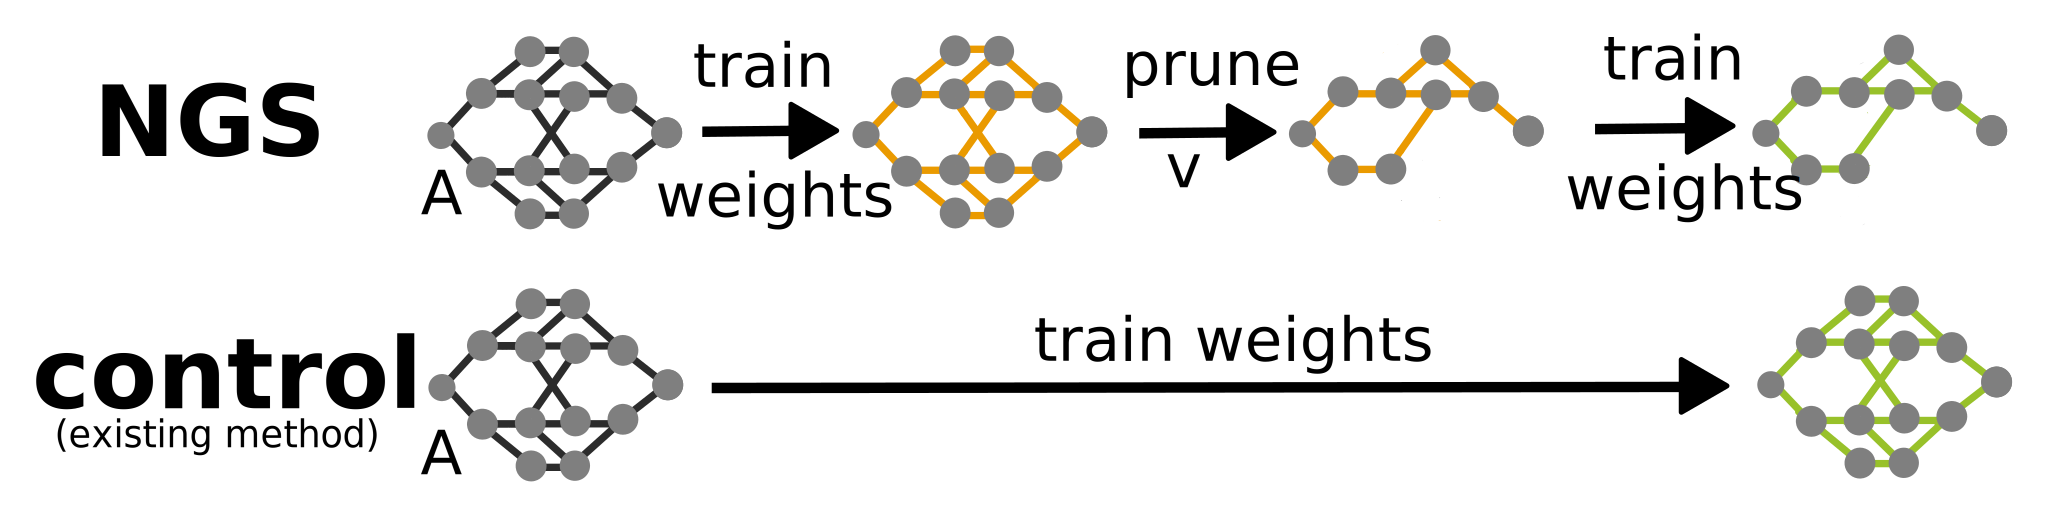
\includegraphics[width=\textwidth]{img/complete}
\end{minipage}%
\begin{minipage}{0.2\textwidth}
  {\setstretch{0.7}
  \begin{footnotesize}
    \textit{
   Figure 1: A schematic comparison of a candidate NGS solution (top) with a candidate solution under existing methods (bottom).
   }
  \end{footnotesize}
  \par}
\end{minipage}

\section{Research Plan}

I will investigate NGS in evolutionary deep learning architecture design in two stages.
First, in smaller scale experiments, I will compare evolvability and irregular refinement metrics under NGS and control treatments. Subsequently, in larger scale experiments, I will demonstrate the utility of NGS on benchmark deep learning datasets.
These experiments will be performed at the High Performance Computing Center at Michigan State University.

Small scale experiments will employ the HyperNEAT encoding,\autocite{clune2011performance} a standard indirect encoding for neuroevolution.
A variant of the bit mirroring problem, which is designed to permit explicit manipulation of problem regularity, will be employed.
Evolvability will be assessed by measuring the phenotypic novelty and viability of mutant offspring of champion candidate architectures.
The capacity of NGS-HyperNEAT to enable irregular refinement will be assessed by comparing control and NGS-HyperNEAT treatment performance across a spectrum of problem regularities.
Greater relative performance of NGS-HyperNEAT at low problem regularity would confirm that NGS enables irregular refinement.

Larger scale experiments will employ the CoDeepNEAT encoding,\autocite{miikkulainen2017evolving} an indirect encoding developed especially for evolving deep learning architectures.
Unlike HyperNEAT, the node-level unit in CoDeepNEAT is an ANN layer (instead of an individual neuron).
I will benchmark NGS-CoDeepNEAT on datasets for computer vision (CIFAR-10/100) and language modeling (PTB).
I expect performance to meet or exceed state-of-the-art.
